\section{Loading data}
\paragraph{}
The image we'll try to apply binarisation to is the following:

\begin{figure}[h]
    \centering
    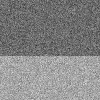
\includegraphics{2classes_100_100_8bits_2016.png}
    \caption{Image to experiment on}
    \label{merged-image}
\end{figure}

\paragraph{}
Which is composed of the following 2 images:

\begin{figure}[h]
    \centering
    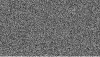
\includegraphics{2classes_100_100_8bits_omega1_2016.png}
    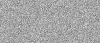
\includegraphics{2classes_100_100_8bits_omega2_2016.png}
    \caption{Separate images}
    \label{separate-images}
\end{figure}

\paragraph{}
The images will be be loaded as gray images:

\begin{lstlisting}[language=R, caption=Loading data in R]
    # Chargement d'une image en niveaux de gris
    rdfReadGreyImage <- function (nom) {
        image <- readImage (nom)
        if (length (dim (image)) == 2) {
            image
        } else {
            channel (image, 'red')
        }
    }   
\end{lstlisting}


\clearpage


\section{Technical acknowledgements}
\paragraph{}
Please note that for the following scripts, some data was pre-loaded to avoid loading it every time.

\begin{lstlisting}[language=R, caption=Loading some data only once]
    # loading some data only once
    image <- rdfReadGreyImage ("2classes_100_100_8bits_2016.png")
    above <- rdfReadGreyImage ("2classes_100_100_8bits_omega1_2016.png")
    below <- rdfReadGreyImage ("2classes_100_100_8bits_omega2_2016.png")

    nbins <- 256
    h <- hist (as.vector (image), freq=FALSE, breaks = seq (0, 1, 1 / nbins))
    h1 <- hist (as.vector (above), freq=FALSE, breaks = seq (0, 1, 1 / nbins))
    h2 <- hist (as.vector (below), freq=FALSE, breaks = seq (0, 1, 1 / nbins))
\end{lstlisting}

\section{Fixed threshold}
\paragraph{}
Let's take a look at the histograms below.
Left is for the ``merged'' image, right is for the separate images, the histograms being plotted together.
Based on the left histogram, we can have a ``manual'' attempt at binarising the image: using a \emph{fixed threshold}.
We simply choose a value for the threshold and we assign, for each pixel, one of the predicted classes as it follows:
$$\hat{w_1} = \{P \in I | I(P) < \hat{X}\}$$
$$\hat{w_2} = \{P \in I | I(P) \ge \hat{X}\}$$
where $\hat{X}$ is our threshold.

\begin{figure}[h]
    \centering
    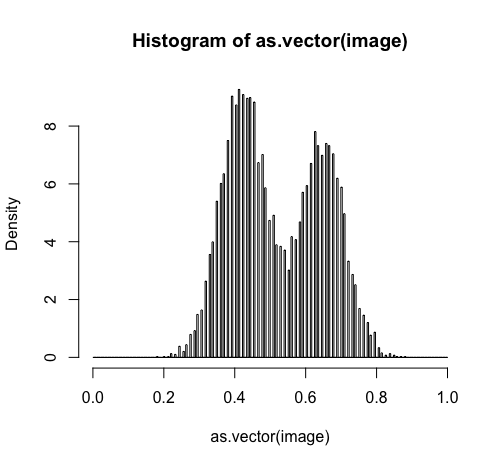
\includegraphics[width=\textwidth/2 - 10pt]{histogram1.png}
    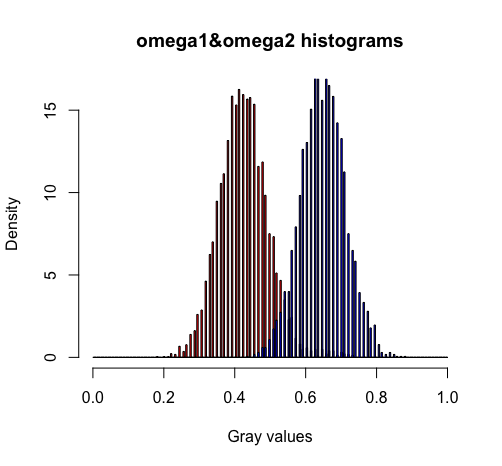
\includegraphics[width=\textwidth/2 - 10pt]{combined_histograms.png}
    \caption{Histogram of grey values for}
    \label{}
\end{figure}

\begin{lstlisting}[language=R, caption=Using fixed threshold]
    # for each threshold, calculate the binary image
    # image has values between [0, 1] so our threshold has to be in the same range
    # for each pixel, the expression (pixel_value - threshold) >= 0 will assign it to one of two classes: w1 or w2
    binaire50 <- (image - 0.5) >= 0
    display (binaire50, "image binaire 0.35", method="raster", all=TRUE)
    binaire55 <- (image - 0.55) >= 0
    display (binaire55, "image binaire 0.35", method="raster", all=TRUE)
    binaire60 <- (image - 0.6) >= 0
    display (binaire60, "image binaire 0.35", method="raster", all=TRUE)
\end{lstlisting}

\clearpage

\paragraph{}
Let's take a look at the results, using threshold values of $0.5$, $0.55$ and $0.6$.

\begin{figure}[h]
    \centering
    
\includegraphics[width=\textwidth/3 - 10pt]{threshold_05.png}
    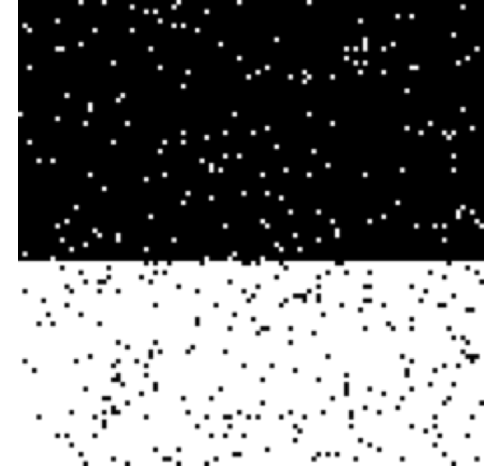
\includegraphics[width=\textwidth/3 - 10pt]{threshold_055.png}
    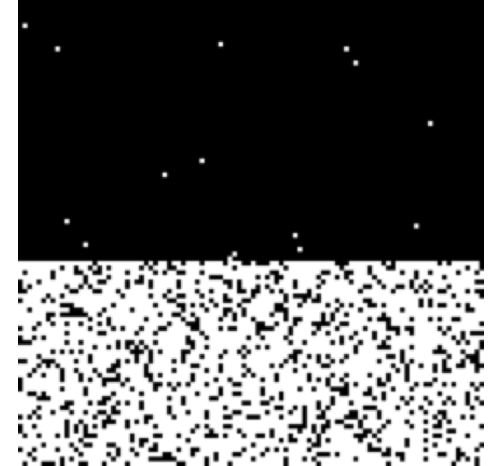
\includegraphics[width=\textwidth/3 - 10pt]{threshold_06.png}
    \caption{Fixed threshold results}
    \label{}
\end{figure}

\paragraph{}
It is not hard to see that there is a lot of noise in our predictions and that they are far from perfect.
The threshold value of $0.6$ might seem attractive, but it only manages to classify well most of the pixels from the image on the top.
Further more, it heavily missclassifies the pixels from the image on the bottom.

\section{A priori class probabilities}
\paragraph{}
Our image \ref{merged-image} is formed of 2 separate images \ref{separate-images}.
We can try to calculate the following probabilities:
\begin{center}
    $P(w_1)$, the probability of a pixel to be in $w_1$ class
    \\
    $P(w_2)$, the probability of a pixel to be in $w_1$ class
\end{center}

\paragraph{}
Knowing that the dimension of the merged image is $100$x$100$ and the 2 images are $100$x$43$, $100$x$57$, the probabilities above are easy to calculate.

\begin{lstlisting}[language=R, caption=A priori class probabilities]
    calculateClassAPrioriProbabilities <- function(){
        # pw1 = (number_of_pixels_from_the_first_image) / (number_of_total_pixels)
        # pw1 = (number_of_pixels_from_the_second_image) / (number_of_total_pixels)
        noTotalPixels = dim(image)[1] * dim(image)[2]
        pw1 = (dim(above)[1] * dim(above)[2]) / noTotalPixels
        pw2 = (dim(below)[1] * dim(below)[2]) / noTotalPixels
        c(pw1, pw2)
    }
\end{lstlisting}

\paragraph{}
In this case, the probabilities are $P(w_1) = 0.57$ and $P(w_2) = 0.43$.

\clearpage

\section{Conditional probabilities}
Having $P(w_1)$ and $P(w_2)$, we can take a step further and calculate the following conditional probabilities:
\begin{center}
    $P(X|w_1)$, the probability of a pixel having the gray value of $X$ if it's in the $w_1$ class
    \\
    $P(X|w_2)$, the probability of a pixel having the gray value of $X$ if it's in the $w_2$ class
\end{center}

\paragraph{}
These are, according to \cite{bayes_theorem}, equal to:
$$P(X|w) = \frac{P(w | X) * P(X)}{P(w)}$$

\paragraph{}
We already have $P(w)$ and $P(X)$ is simply the number of pixels with the gray value of $X$ divided by the total number of pixels.
$P(w | X)$ is the number of pixels with the value $X$ in the merged image corresponding to $w$ divided by the total number of pixels with a value of $X$.

\begin{lstlisting}[language=R, caption=Calculating conditional probabilities]
    calculateConditionalProbability <- function (X, probs){
        # let's take a look at the histogram again
        # we can notice that h$counts[X + 1] gives us the number of pixels that have the gray value of X
        # the "+ 1" above is because in R arrays start from 1

        # so, P(X | I) = the probability of a pixel from the merged image to have the gray value of X
        px <- h$counts[X + 1] / sum(h$counts)
        # P(X | w) = the probability of a pixel from the merged image to have the gray value of X
        # IF that pixel is from the w class
        # Using bayes theorem, we get:
        # P(X|w) = (P(w | X) * P(X)) / P(w)
        # and P(w | X) = how many pixels of value X are in the image corresponding to w / the total number of pixels with a value of X

        p_w1_if_x <- h1$counts[X + 1] / h$counts[X + 1]
        p_x_and_w1 <- p_w1_if_x * px
        p_x_if_w1 <- p_x_and_w1 / probs[1]

        p_w2_if_x <- h2$counts[X + 1] / h$counts[X + 1]
        p_x_and_w2 <- p_w2_if_x * px
        p_x_if_w2 <- p_x_and_w2 / probs[2]

        c(px, p_x_if_w1, p_x_if_w2)
    }

    print (calculateConditionalProbability(141, probs))
\end{lstlisting}

\paragraph{}
Running the above function for $X=141$, we get the following probabilities:
\begin{center}
    $P(X|I) = 0.011800000$
    \\
    $P(X|w_1) = 0.008947368$
    \\
    $P(X|w_2) = 0.015581395$
\end{center}
where $P(X|I)$ refers to the probability of a pixel to have the gray value of $X$ in the whole (merged) image. Of course, $P(X|w_1) * P(w_1) + P(X|w_2) * P(w_2) = P(X|I)$.

\clearpage

\section{Automatic thresholding using Bayes}

\paragraph{}
Having a threshold $\hat{X}$, we can define an assignment error as being the following:
$$P(\epsilon | \hat{X}) = \underset{x}{\operatorname{argmin}}
(
\underset{X\in\hat{w_2}}{\sum} P(X|w_1) * P(w_1)
+
\underset{X\in\hat{w_1}}{\sum} P(X|w_2) * P(w_2)
)
$$
\paragraph{}
Our goal is to find the $\hat{X}$ that minimizes $P(\epsilon | \hat{X})$.
For this, we can try each value for $\hat{X}$ and see which is the best.

\begin{lstlisting}[language=R, caption=Automatic segmentation using Bayes]
    automaticSegmentationUsingBayes <- function(){
        # calculate these probabilities only once
        probs <- calculateClassAPrioriProbabilities()
        # only get the imageData, it will be faster for comparisons
        image <- imageData(image)
        # build our reference segmentation
        perfect <- matrix (nrow=dim(image)[1], ncol=dim(image)[2])
        # dim(image)[1] = number of columns
        for (i in 1:dim(image)[1])
          for (j in 1:dim(above)[2]){
            perfect[i, j] <- FALSE
          }
        for (i in 1:dim(image)[1])
          for (j in dim(above)[2]:dim(image)[2]){
            perfect[i, j] <- TRUE
          }
        display(perfect, method="raster", all=TRUE)
        
        # precalculate all probabilities
        condProbs <- matrix(nrow = 256, ncol = 2)
        for (X in 0:255){
          res <- calculateConditionalProbability(X, probs)
          condProbs[X + 1, 1] <- res[2]
          condProbs[X + 1, 2] <- res[3]
        }
        
        min_error = 2 * dim(image)[1] * dim(image)[2]
        for (X in 0:255){
          binary <- (image - X/255) >= 0
          # only get the data, otherwise the comparisons will be really slow
          binary <- imageData(binary)
          error <- 0
          # these pixels should be in w1 class
          for (i in 1:dim(image)[1])
            for (j in 1:dim(image)[2])
              if (perfect [i, j] != binary [i, j]){
                # if it should be in the first class
                if (j < dim(above)[2])
                  error <- error + condProbs[image[i, j] * 255 + 1, 1] * probs[1]
                else
                  error <- error + condProbs[image[i, j] * 255 + 1, 2] * probs[2]
              }
          if (error < min_error){
            min_error <- error
            best_threshold <- X
          }
        }
        print (c(min_error, best_threshold))
        # segment using best_threshold
        binary <- (image - best_threshold/255) >= 0
        display(binary, method="raster", all=TRUE)
      }
\end{lstlisting}

\paragraph{}
Below we can look at the ``perfect'' image and the one we got using this automatic segmentation.
To calculate the ``perfect'' segmentation, we simply assigned all pixels from the first (above) image to a class, and the rest to another class.
According to the script, the minimum error is $1.636$ and the best threshold for the gray value is $X = 139$.

\begin{figure}[h]
    \centering
    
\includegraphics[width=\textwidth/2 - 10pt]{perfect.png}
    
\includegraphics[width=\textwidth/2 - 10pt]{best_segmentation.png}
    \caption{Perfect segmentation and our best result}
    \label{}
\end{figure}


\section{Segmenting digits}
\paragraph{}
We'll take a look now at the results of this method for some digits. We'll be working with the following images:

\begin{figure}[h]
    \centering
    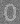
\includegraphics{rdf-chiffre-0-8bits.png}
    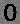
\includegraphics{rdf-chiffre-0-8bits_omega1.png}
    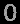
\includegraphics{rdf-chiffre-0-8bits_omega2.png}
    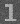
\includegraphics{rdf-chiffre-1-8bits.png}
    
\includegraphics{rdf-chiffre-1-8bits_classe_a_trouver.png}
    \caption{Digit images}
    \label{}
\end{figure}

\paragraph{}
For the $0$ digit, we have 3 images: one we need to segment and 2 already ``segmented'' photos.
For the second and third segment, we can see that some pixels are black. Those pixels correspond to the $w_1$ and $w_2$ classes.
We'll be using this fact for the calculation of probabilities.

\paragraph{}
Let us first load our new new data and work with the $0$ digit:
\begin{lstlisting}[language=R, caption=Loading data for digits]
    # get img, w1 and w2 histograms
    image <- rdfReadGreyImage("rdf-chiffre-0-8bits.png")
    img_w1 <- rdfReadGreyImage("rdf-chiffre-0-8bits_omega1.png")
    img_w2 <- rdfReadGreyImage("rdf-chiffre-0-8bits_omega2.png")
    nbins <- 256
    h <- hist (as.vector (image), freq=FALSE, breaks = seq (0, 1, 1 / nbins))
    h1 <- hist (as.vector (img_w1), freq=FALSE, breaks = seq (0, 1, 1 / nbins))
    h2 <- hist (as.vector (img_w2), freq=FALSE, breaks = seq (0, 1, 1 / nbins))
\end{lstlisting}

\clearpage

\paragraph{}
To use the automatic bayes thresholding, we need to calculate $P(w)$, $P(X)$ and $P(X|w)$, so $P(w|X)$ as well.
$P(w)$ will be equal to the number of pixels from the $w$ class (so the black pixels in the second and third images) divided by the total number of pixels.
For $P(X)$, we simply divide the number of pixels with the gray value of $X$ to the total number of pixels.
\paragraph{}
$P(w|X)$ isn't that tricky.
If, for example, the pixels of value $X$ belong to the $w_1$ class, then in the histogram for $w_1$ we won't have any $X$ values.
That's because those pixels with the value of $X$ were given the $0$ value (black pixels).
\paragraph{}
So, $\frac{count_{total} - count_{w_1}} {count_{total}}$ will give us the proportion of pixels of value $X$ that were assigned to the $w_1$ class.
We can use this to calculate $P(w|X)$. Afterwards, we can easily calculate $P(X|w)$ using Bayes' theorem.

\begin{lstlisting}[language=R, caption=Automatic segmentation for digit 0]
    classify0Digit <- function(){
        # calculate a priori probabilities
        # P(w) = probability of a pixel to be in the w class
        # the pixels that are in w class have a gray value of 0 in the image corresponding to w
        probs <- c(h1$counts[1] / sum(h$counts), h2$counts[1] / sum(h$counts))
        
        # only get the imageData, it will be faster for comparisons
        image <- imageData(image)
        img_w1 <- imageData(img_w1)
        img_w2 <- imageData(img_w2)
        
        # build our reference segmentation
        perfect <- matrix (nrow=dim(image)[1], ncol=dim(image)[2])
        # dim(image)[1] = number of columns
        for (i in 1:dim(image)[1])
          for (j in 1:dim(image)[2]){
            if (img_w1[i, j] == 0){
              perfect[i, j] <- TRUE
            }
            else{
              perfect[i, j] <- FALSE
            }
          }
        display(perfect, method="raster", all=TRUE)
        
        # precalculate all conditional probabilities
        condProbs <- matrix(nrow = 256, ncol = 2)
        for (X in 0:255){
          px <- h$counts[X + 1] / sum(h$counts)
          # P(X | w) = probability of a pixel having the gray value of X if the pixel is from class w
          # Using bayes theorem, we get:
          # P(X|w) = (P(w | X) * P(X)) / P(w)
          # P(w | X) = the prob. of the pixel being from the w class, if its value is X
          # 
          
          # h1$counts[X + 1] + h2$counts[X + 1] = h$counts[X + 1]
          # if h1$counts[X + 1] - h$counts[X + 1] is different than 0, then those pixels were NOT assigned to w1
          
          if (px == 0){
            condProbs[X + 1, 1] <- 0
            condProbs[X + 1, 2] <- 0
            next
          }
          p_w1_if_x <- (h$counts[X + 1] - h1$counts[X + 1]) / h$counts[X + 1]
          p_x_and_w1 <- p_w1_if_x * px
          p_x_if_w1 <- p_x_and_w1 / probs[1]
          p_w2_if_x <- (h$counts[X + 1] - h2$counts[X + 1]) / h$counts[X + 1]
          p_x_and_w2 <- p_w2_if_x * px
          p_x_if_w2 <- p_x_and_w2 / probs[2]
          
          condProbs[X + 1, 1] <- p_x_if_w1
          condProbs[X + 1, 2] <- p_x_if_w2
        }
        
        probSum <- 0
        for (X in 0:255){
          if(is.nan(condProbs[X + 1, 1]) == FALSE)
            probSum <- probSum + probs[1] * condProbs[X + 1, 1] + probs[2] * condProbs[X + 1, 2]
        }
        
        print ('Making sure that the sum of conditional probabilities is 1:')
        print (probSum)
      
        # search for the best threshold
        min_error <- 2 * dim(image)[1] * dim(image)[2]
        best_threshold <- 0
        for (X in 0:255){
          binary <- (image - X/255) >= 0
          # only get the data, otherwise the comparisons will be really slow
          binary <- imageData(binary)
          
          error <- 0
          for (i in 1:dim(image)[1])
            for (j in 1:dim(image)[2])
              if (perfect [i, j] != binary [i, j]){
                # if it should have been in w1
                if (img_w1[i, j] == 0)
                  error <- error + condProbs[image[i, j] * 255 + 1, 1] * probs[1]
                else
                  # it should have been in w1
                  error <- error + condProbs[image[i, j] * 255 + 1, 2] * probs[2]
              }
          
          if (error < min_error){
            min_error <- error
            best_threshold <- X
          }
        }
        print (c (min_error, best_threshold))
        # segment using best_threshold
        binary <- (image - best_threshold / 255) >= 0
        display(binary, method="raster", all=TRUE)
    }
\end{lstlisting}

\clearpage

\paragraph{}
Running the above script will give us an error of $0.04583333$, the best threshold being $X=142$.
We also applied the same threshold for digit $1$ and we can see that it is quite a good threshold.
The segmentation isn't perfect, but it gets the job done.

\begin{figure}[h]
    \centering
    
\includegraphics[width=72px]{0_segmentation.png}
    
\includegraphics[width=72px]{1_segmentation.png}
    \caption{Automatic segmentation using best treshold for digit $0$}
    \label{}
\end{figure}

\begin{figure}[h]
    \centering
    
\includegraphics[width=72px]{0_perfect.png}
    
\includegraphics[scale=3]{rdf-chiffre-1-8bits_classe_a_trouver.png}
    \caption{Perfect segmentation}
    \label{}
\end{figure}


\section{Classification error}
As a final conclusion, we can look at the error rate of our algorithm.

\begin{lstlisting}[language=R, caption=Calculating error rate]
    binary <- (image - best_threshold / 255) >= 0
    # build our reference segmentation
    perfect <- matrix (nrow=dim(image)[1], ncol=dim(image)[2])
    # dim(image)[1] = number of columns
    for (i in 1:dim(image)[1])
      for (j in 1:dim(image)[2]){
        if (img_w1[i, j] == 0){
          perfect[i, j] <- TRUE
        }
        else{
          perfect[i, j] <- FALSE
        }
      }
    sprintf("Error for digit 0: %f", sum(abs(perfect - binary)) / (dim(perfect)[1] * dim(perfect)[2]))
    
    # calculate error rate for 1
    image <- rdfReadGreyImage("rdf-chiffre-1-8bits.png")
    binary <- (image - best_threshold / 255) < 0
    perfect <- rdfReadGreyImage("rdf-chiffre-1-8bits_classe_a_trouver.png")
    display(binary, method="raster", all=TRUE)
    sprintf("Error for digit 1: %f", sum(abs(perfect - binary)) / (dim(perfect)[1] * dim(perfect)[2]))
    
\end{lstlisting}

\paragraph{}
This gave us an error rate of $0.033333$, that is around $3.3\%$ missclassified pixels for digit $0$.
For digit $1$, we have an error of $0.029167$, so around $3\%$ missclassified pixels.

